%==========================オプションおよび文書クラスの設定==========================
%"autodetect-engine"-どのエンジンでもコンパイル可能にするオプション
%"dvipdfmx-if-dvi"-必要な場合のみdvipdfmx経由のpdf化をするオプション(LuaTeXやXeTeXはPDFに直接変換するため)
%"ja=standard"-日本語文書の標準設定を利用するオプション
%"bxjs…"-どのエンジンでも利用可能なドキュメントクラス
%--以下のいずれかを選択--
\documentclass[autodetect-engine,dvipdfmx-if-dvi,ja=standard,a4paper,11pt]{bxjsarticle} %章の無いレポート
%\documentclass[autodetect-engine,dvipdfmx-if-dvi,ja=standard,a4paper,10pt]{bxjsslide} %スライド
%\documentclass[autodetect-engine,dvipdfmx-if-dvi,ja=standard,a4paper,10pt]{bxjsbook} %書籍
%\documentclass[autodetect-engine,dvipdfmx-if-dvi,ja=standard,a4paper,10pt]{bxjsreport} %章のある論文やレポート

%==============================プリアンブルの設定==============================
\title{春期課題} %タイトル
\author{新B4 福田真悟} %著者名
\date{2020.3.3}%日付 %日付下の余白をN[mm]減らす

%///////////////////////////////////////////////////////////////////////////////////////////////////////////
%////////////////////////////////////パッケージの読込み及び設定の書換え//////////////////////////////////////
%///////////////////////////////////////////////////////////////////////////////////////////////////////////
\usepackage{graphicx} %図の挿入に関するパッケージ
\usepackage{float} %[H]で図の位置を固定する機能をONにするパッケージ
\usepackage{subcaption} %サブキャプションに関するパッケージ
\captionsetup{labelsep=space} %サブキャプション後の":"を非表示にする
\usepackage{enumerate} %{enumerate}[]の,[]の中の通りの箇条書きにすることができるパッケージ
\usepackage{amsmath} %数式に関するパッケージ
\usepackage{mathtools} %数式に関するパッケージ
\usepackage{bm} %ベクトル表示のコマンドを追加するパッケージ
\usepackage{comment} %複数行のコメントアウトを可能にするパッケージ
\usepackage{ascmac} %枠に関するパッケージ
\usepackage{tabularx} %表に関するパッケージ
\setpagelayout{top=10truemm,bottom=15truemm,left=15truemm,right=15truemm}  %余白に関する設定の書換え(bxjs…クラスではgeometryパッケージは使用不可)
\graphicspath{{../figures/}} %図を挿入する際に.texファイルの上の階層にあるfiguresというフォルダを参照可能にする
\usepackage{url}

%余白に関する設定の書換え(bxjs…クラスではgeometryパッケージは使用不可)
\belowcaptionskip=-0pt %キャプション下の余白をN[pt]減らす
\graphicspath{{../figures/}} %図を挿入する際に.texファイルの上の階層にあるfiguresというフォルダを参照可能にする

%使用記号の追加
\newcommand{\divergence}{\mathrm{div}\,}  %ダイバー
\newcommand{\grad}{\mathrm{grad}\,}  %グラディエント
\newcommand{\rot}{\mathrm{rot}\,}  %ローテーション

%\pagestyle{myheadings} %myheading文字列 emptyページ番号なし plainフッダーに
%\markright{\footnotesize 2月28日(金)15:00~ 顔合わせ}%全ページ共通への挿入
%================================以下本文================================
\begin{document}
\maketitle %設定したタイトルの挿入
\section{\normalsize"Lorenz 方程式","Rossler 方程式","ホワイトガウスノイズ","Logistic 写像"
,"順列エントロピー","相互情報量","複雑ネットワーク"について書籍やインターネットで調べる
}%sectionの前に*をつけると数字の振り分けが消える不思議


\begin{itemize}
\item Lorenz 方程式\\
カオス的なふるまいを示す非線形微分方程式の1つで
\begin{equation}
\frac{dx}{dt}=-px+py
\end{equation}
\begin{equation}
\frac{dy}{dt}=-xz+rx-y
\end{equation}
\begin{equation}
\frac{dz}{dt}=xy-bz
\end{equation}
で表現される \cite{lo} .変数は$(x,y,z,t)$,定数は$(p,r,b)$である.初期値鋭敏性から初期値によって,それ以降の結果が大きく変化してしまう.そのため初期値の精度には無限大の精度が必要となり,予測が事実上不可能となっている.

\begin{figure}[H]%[h]は記述したところ。[t]はそのページの上端。[t]はそのページの下端、[p]はページいっぱい
\begin{center}

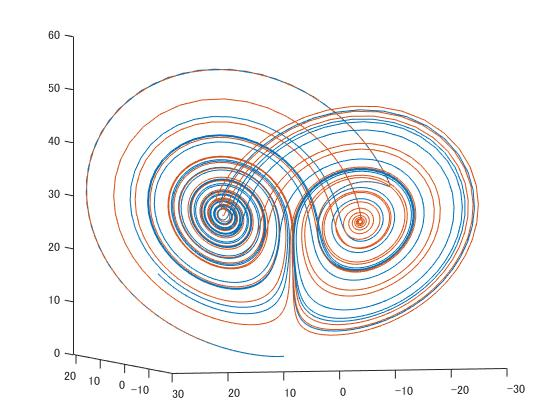
\includegraphics[width=.4\textwidth]{Lorenz_result.jpg}
\end{center}
\caption{Lorenz方程式の誤差の増幅}%図名
\label{fig:lorenz}
\end{figure}

図 \ref{fig:lorenz}は初期値の1つを0.1変化させたときの解の変化である.

\item Rossler 方程式\\
カオス的なふるまいを示す非線形微分方程式の1つで
\begin{equation}
\frac{dx}{dt}=-y-z
\end{equation}
\begin{equation}
\frac{dy}{dt}=x+ay
\end{equation}
\begin{equation}
\frac{dz}{dt}=b+xz-cz
\end{equation}
で表現される \cite{re} .変数は$(x,y,z,t)$,定数は$(a,b,c)$である.Lorenz方程式と違い,カオスの挙動を把握するために単純化された方程式であり,実際の物理モデルがベースではない.Lorenz方程式と同様に初期値鋭敏性から初期値によって,それ以降の結果が大きく変化してしまう.そのため初期値の精度には無限大の精度が必要となり,予測が事実上不可能となっている.

\begin{figure}[H]%[h]は記述したところ。[t]はそのページの上端。[t]はそのページの下端、[p]はページいっぱい
\begin{center}
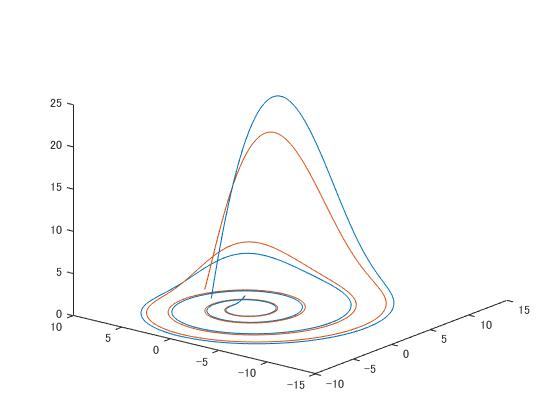
\includegraphics[width=.4\textwidth]{Rossler_result.jpg}
\end{center}
\caption{Rossler方程式の誤差の増幅}%図名
\label{fig:rossler}
\end{figure}

図 \ref{fig:rossler}は初期値の1つを0.1変化させたときの解の変化である.


\item ホワイトガウスノイズ\\
自然界などのランダム過程の効果をモデル化したもの.ホワイトは周波数帯域が均一であることを示している.光の白色から由来している.ガウスは自然界のものはガウス分布に従うという仮定をもとにノイズもガウス分布となっていることを示している.波形の周波数は均一にすべての周波数で,波形の振幅はガウス分布に従う振幅となっていると仮定したノイズ.

\item Logistic 写像\\
Logistic方程式を離散化することで得られる漸化式である.
\begin{equation}
x_{n+1}=ax_{n}(1-x_{n})
\end{equation}
定数$a$によって,値の変化が大きく変わる.$a$が十分に小さいときは0に収束し,値が大きくなるにつれて,収束値が大きくなり,周期的な振動を示し,最終的にカオス的な挙動を示す.$a$ごとの$x$の値の変化を下記に示す.

\begin{figure}[H]%[h]は記述したところ。[t]はそのページの上端。[t]はそのページの下端、[p]はページいっぱい
\begin{center}
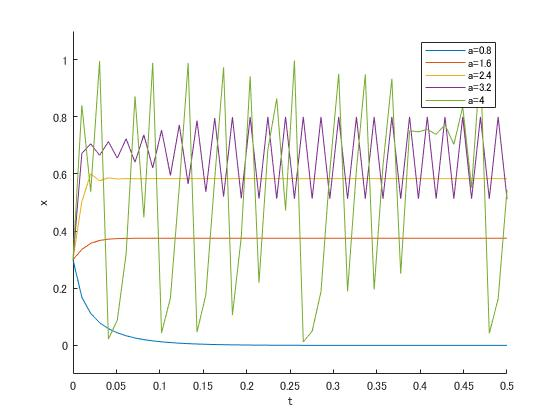
\includegraphics[width=.4\textwidth]{Logistic_result.jpg}
\end{center}
\caption{$a$の変化によるLogistic写像の値の変化}%図名
\label{fig:logstic}
\end{figure}


\item 順列エントロピー\\


\item 相互情報量\\

\item 複雑ネットワーク\\

\end{itemize}


\section{\normalsize相互情報量とLorenz 方程式に関するMATLAB ファイル(mutual.m) を実行し,図を出力する}
出力された結果を下記に示す.

\begin{figure}[H]%[h]は記述したところ。[t]はそのページの上端。[t]はそのページの下端、[p]はページいっぱい
\begin{center}
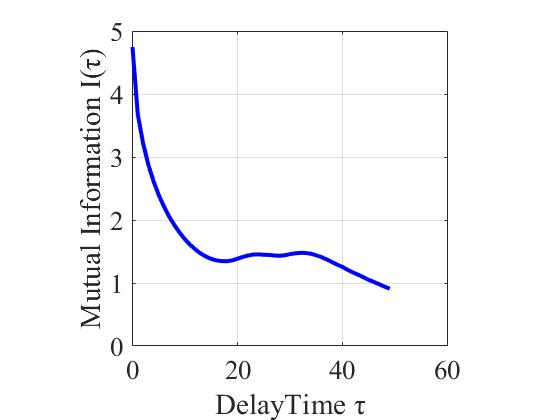
\includegraphics[width=.4\textwidth]{kadai2_rusult.jpg}
\end{center}
\caption{課題2の出力結果}%図名
\label{fig:kadai2}
\end{figure}


\section{\normalsizeホワイトガウスノイズと順列エントロピーに関するMATLABファイル(B4kadai\_2020.m)を実行し,図を出力し考察を加える.}
まず出力された結果を下記に示す.

\begin{figure}[H]%[h]は記述したところ。[t]はそのページの上端。[t]はそのページの下端、[p]はページいっぱい
\begin{center}
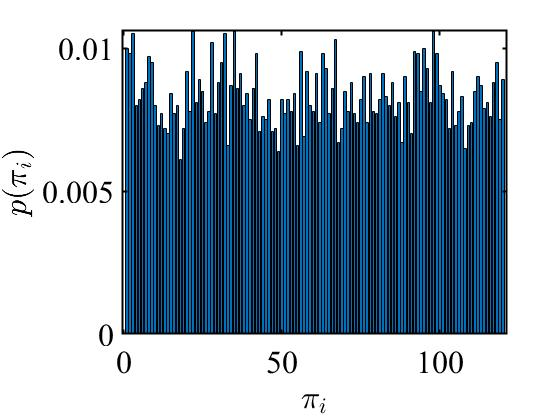
\includegraphics[width=.4\textwidth]{kadai3_rusult.jpg}
\end{center}
\caption{課題3の出力結果}%図名
\label{fig:kadai3}
\end{figure}



%$A^1$\cite{aaa}%参考文献




%\begin{itemize}
%\item アイテムコード1
%\item アイテムコード2
%\item アイテムコード3
%\item アイテムコード4
%\item アイテムコード5
%\end{itemize}


%\begin{figure}[H]%[h]は記述したところ。[t]はそのページの上端。[t]はそのページの下端、[p]はページいっぱい
%\begin{center}
%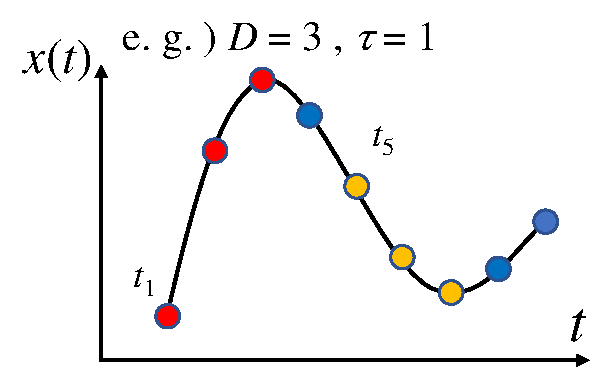
\includegraphics[width=.4\textwidth]{crop_PE1ver2.pdf} 
%\end{center}
%\caption{時系列$ x(t) $}%図名
%\label{fig:PE1}%fig図tb表
%\end{figure}



\begin{thebibliography}{9999}%参考文献
\bibitem{lo}%参考文献citeするぞ
ローレンツ方程式,\url{http://www.isc.meiji.ac.jp/~random/lecture/2015-comp2/Lorentz_equ.html}
\bibitem{re}
カオス・フラクタル\ 講義ノート\ \#8,\url{https://ocw.hokudai.ac.jp/wp-content/uploads/2016/01/ChaosFractal-2011-Note-08.pdf}
\bibitem{lo}%参考文献citeするぞ
ローレンツ方程式,\url{http://www.isc.meiji.ac.jp/~random/lecture/2015-comp2/Lorentz_equ.html}
\bibitem{re}
カオス・フラクタル\ 講義ノート\ \#8,\url{https://ocw.hokudai.ac.jp/wp-content/uploads/2016/01/ChaosFractal-2011-Note-08.pdf}

\end{thebibliography}

%\newpage



\end{document}